\section{Métodos}
\label{sec:3}

La metodología se basa en observación en terreno y experimentos a escala real. Para estudiar las puertas en andén se escogió dos estaciones de la Línea 6 del Metro de Santiago. Tal como se observa en la Ilustración 1, la estación Ñuñoa cuenta con dichas puertas, pero no posee demarcación en el andén. Por otro lado, la estación Ñuble cuenta con puertas en andén y demarcación para indicar donde se ubican. 

\begin{figure}[h]
  \centering
  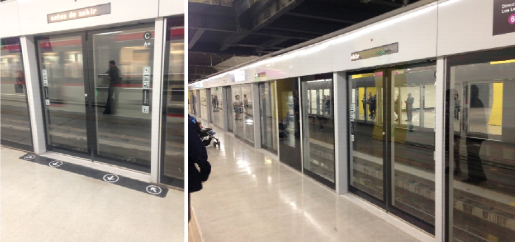
\includegraphics[width=0.8\textwidth]{imagenes/ilustracion_1.png}
  \caption{Puertas en andén con demarcación en estación Ñuble (izquierda) y sin demarcación en estación Ñuñoa (derecha), Línea 6, Metro de Santiago}\label{fig1}
\end{figure}

Ambas estaciones se observaron en noviembre 2018 durante tres días hábiles mediante el uso de cámaras de video ubicadas a 4 m de altura justo arriba de la puerta de andén más utilizada. Se pudo reportar que ambas estaciones poseen una demanda similar de pasajeros que suben y bajan del tren. En la hora punta en Ñuñoa se observó en promedio 13 pasajeros que suben y 9 pasajeros que bajan, lo que equivale a una razón (R) de pasajeros que suben con respecto a los que bajan de 1,6. En el caso de Ñuble en la hora punta se observó en promedio 9 pasajeros que suben y 10 pasajeros que bajan, obteniendo un R = 1. El cálculo de R se obtiene mediante la división entre el número total de pasajeros que sube y el número total de pasajeros que baja.

Para medir el efecto de la demarcación en las puertas en andén, se utilizó un modelo conceptual en donde se discretizó la interfaz tren-andén en celdas cuadras de 40 cm de ancho. Cada celda representa el tamaño de la baldosa del suelo del andén. El supuesto es que cada celda es utilizada por un pasajero que espera la llegada del tren (ver Ilustración 2). Esta forma de dividir la interfaz permite identificar lo siguiente:
\begin{itemize}
  \item La celda más utilizada, al contar el número de veces que un pasajero pasa por una celda durante la hora punta observada en cada estación. 
  \item Ubicación de los pasajeros que esperan subir al tren (frente a las puertas o a los costados de estas).
  \item El efecto en los tiempos de subida y bajada para cada caso. En el caso del tiempo de subida se calculó la diferencia entre el último pasajero que sube y el primero que sube. El mismo cálculo se realizó para la bajada. Además, se calculó el tiempo de subida por pasajero haciendo la división entre el tiempo de subida y el número de pasajeros que suben. Lo mismo se calculó para el tiempo de bajada por pasajero.
  \item El efecto en la formación de filas de flujo para pasajeros que bajan del tren.
  \item La posición de los pasajeros dentro del tren no fue analizada en este estudio, sin embargo se considerará como futura investigación.
\end{itemize}

Para estudiar la accesibilidad se consideró la Línea 1 del Metro de Santiago, la cual incluye 27 estaciones subterráneas y 20,4 km de longitud, siendo la más antigua y la que mayor demanda posee con casi un 40\% de toda la red (Metro de Santiago, 2017). Se observó la accesibilidad durante la hora valle para poder medir 8 variables en la interfaz tren-andén. Las variables seleccionadas fueron acordadas con el equipo de Metro de Santiago tomando como base el estudio de Amestoy (2015), la Ley de Accesibilidad Universal (2010) y los estándares del Metro de Londres (2012). La Tabla 1 muestra las variables seleccionadas para medir la accesibilidad.

\begin{figure}[h]
  \centering
  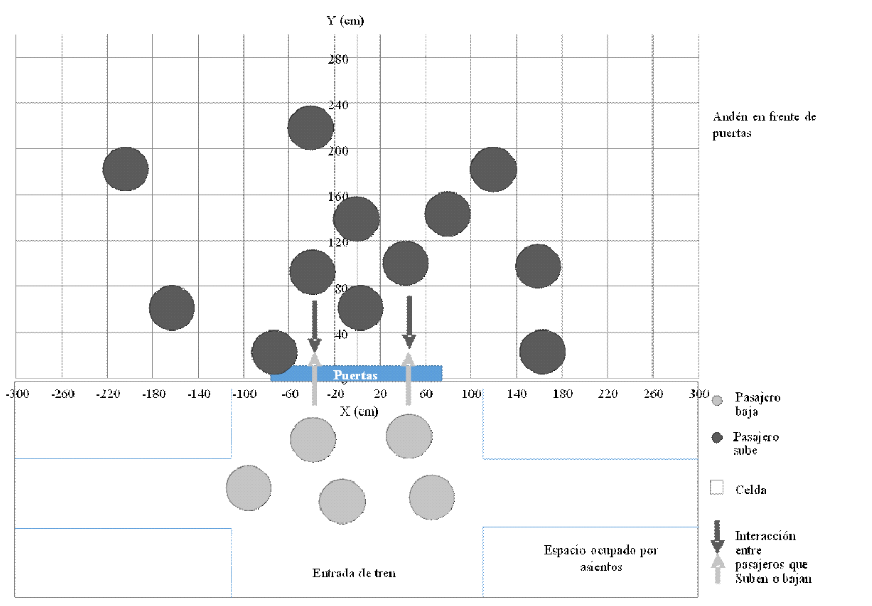
\includegraphics[width=0.8\textwidth]{imagenes/ilustracion_2.png}
  \caption{Modelo conceptual de la interfaz tren-andén discretizado al frente de las puertas}\label{fig2}
\end{figure}


\begin{table}[ht]
  \begin{tabularx}{\linewidth}{|X |X |X|}
  \hline
    Variable & 
    Criterio &
    Fuente \\ 
  \hline
    Espesor de línea amarilla con banda táctil&
    Debe ser de 24 cm, tener podos y color amarillo &
    Amestoy (2015)\\
  \hline
    Distancia entre el borde del andén y la línea amarilla &
    Debe ser mayor a 0,8 m &
    Amestoy (2015)\\
  \hline
    Pavimento guía en andén &
    Debe incluir franjas longitudinales de 0,4 m de ancho &
    DS 50 de Ley Accesibilidad Universal (2010) \\
   \hline
    Pavimento alerta en andén (táctil) &
    Debe tener textura de podos y ancho de 0,4 - 0,8 m &
    DS 50 de Ley Accesibilidad Universal (2010) \\
  \hline
    Ancho de andén &
    Debe ser mayor a 3,0 m &
    Metro de Londres (2012) \\
    \hline
    
    Asientos en andén &
    Debe tener capacidad y diseño accesible &
    Amestoy (2015) \\
    \hline
    
    Intercomunicador en andén &
    Debe ser a una altura no mayor de 1,2 m &
    DS 50 de Ley Accesibilidad Universal (2010) \\
    \hline

    Ascensor &
    Debe tener capacidad para transportar personas con movilidad reducida &
    DS 50 de Ley Accesibilidad Universal (2010) \\
    \hline
  \end{tabularx}
  \caption{Variables seleccionadas para medir la accesibilidad en la interfaz tren-andén}
  \label{tabla1}
\end{table}


Luego de la observación en terreno, \ref{tabla1} se definió una métrica de evaluación en las estaciones estudiadas. Se consideró que todas las variables son igual de importantes, y por ende poseen el mismo ponderador. El ponderador permitió ver cuánto porcentaje de accesibilidad posee cada estación observada en Línea 1. Como existen 8 variables, entonces cada una de ellas representa un 12,5\%. Entonces, por ejemplo, si una estación cumple solo con 4 variables, tendrá un 50\% de accesibilidad. Es decir, el porcentaje de cumplimiento se va sumando a medida que las variables van cumpliendo en la observación realizada.

Finalmente, se realizó un experimento en el Laboratorio de Dinámica Humana (LDH) de la Universidad de los Andes para simular diferentes configuraciones de línea amarilla. En dicho experimento se incluyó personas con discapacidad o movilidad reducida, en donde 2 personas eran de edad avanzada, de las cuales una de ellas padecía de hemiparesia, la que se define como una enfermedad, que técnicamente, es una disminución del movimiento sin llegar a la parálisis en alguna extremidad o lado del cuerpo (sordera y otros problemas auditivos). Además, se contó con una persona con silla de ruedas y una persona que usaba un coche para guaguas (ambos eran jóvenes de 24 años). A estas 4 personas, se consideró otras 21 personas quienes eran estudiantes sin problemas de discapacidad o movilidad, tendiendo así un total de 25 personas que suben y bajan del tren. De los 25 voluntarios, 8 utilizaban el Metro de Santiago cinco o más veces a la semana, es decir un 32\%, incluyendo en este grupo a la persona en silla de ruedas y la persona con hemiparesia, lo cual es importante destacar. Los participantes generaron una densidad en el andén de 4 personas por metro cuadrado, la cual se mantuvo durante las 10 repeticiones por escenario. Con el fin de que la prueba fuese más similar a la realidad del Metro, se le entregó a cada voluntario un número antes de iniciar el experimento, para luego nombrar 5 números elegidos aleatoriamente antes de iniciar cada repetición, con el fin de que los pasajeros con los números escogidos debiesen desplazarse de manera “apurada” al momento de subir al andén e ingresar al tren. Estos pasajeros fueron variando para repetición de subida y bajada.

Respecto a los escenarios de simulación, se probaron 4 casos de espesor de línea amarilla: 5 cm (cinta adhesiva amarilla), 10 cm (doble cinta adhesiva amarilla), 24 cm (PVC con podos amarillos) y 40 cm (carbono y fibra de vidrio reforzada con podos amarillos). Los primeros 3 casos están basados en observación existente en la Línea 1 del Metro de Santiago. Sin embargo, se quiso probar un cuarto espesor (40 cm), para ver un nuevo diseño de línea amarilla. En todos los casos se dejó una distancia entre el borde del andén y la línea amarilla de 1 m (incluyendo el espesor de la línea amarilla). De esta manera, en el caso de un espesor de 40 cm, se mantendría la distancia de seguridad establecida por Metro de Santiago de 60 cm hasta el borde del andén. 

Para determinar cuál de estos escenarios es más efectivo se midió lo siguiente:

\begin{itemize}
  \item Se observó la cantidad de veces que se respetaba la línea amarilla, considerando cuando una persona cruzaba antes de que se diera la instrucción de abrir puertas del tren.
  \item Al finalizar el experimento los participantes debían llenar una encuesta para registrar su experiencia indicando que tan seguro y cómodo se sintió. 
  
\end{itemize}


Con el fin de saber cuál fue la línea que más se respetó en la experimentación, se utilizó la Tabla 2 de evaluación la cual muestra el nivel de cumplimiento que hay por parte de los pasajeros hacia la línea amarilla (Metro de Londres, 2015).

\begin{figure}
  \centering
  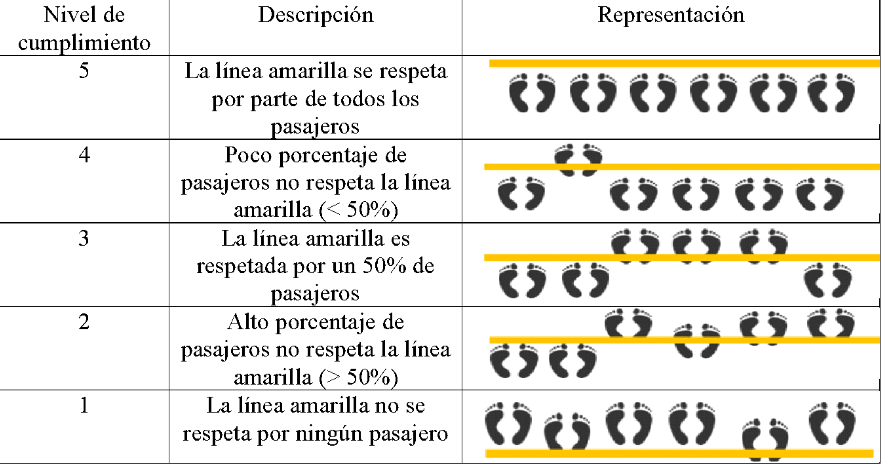
\includegraphics[width=0.8\textwidth]{imagenes/ilustracion_3.png}
  \caption{Tabla Nivel de cumplimiento por parte de los pasajeros (adaptado de Metro de Londres, 2015)
  }\label{fig3}
\end{figure}


En el experimento, la maqueta del vagón es de 2,5 m de ancho por 3 m de largo. Las puertas representan el ancho de la Línea 1 del Metro de Santiago, es decir, 1,65 m. El andén es de 3 m de largo por 3 m de ancho. Para que las personas con movilidad reducida pudieran ingresar al andén se construyó una rampa de acceso. Las cámaras de video se instalaron a 2,5 m en el techo del laboratorio (visión desde arriba) y a 2 m de distancia desde el andén (visión lateral). Estas cámaras permitieron observar la posición de los participantes, la cual fue procesada mediante inteligencia artificial para el conteo automático (ver Ilustración \ref{fig4}).

\begin{figure}
  \centering
  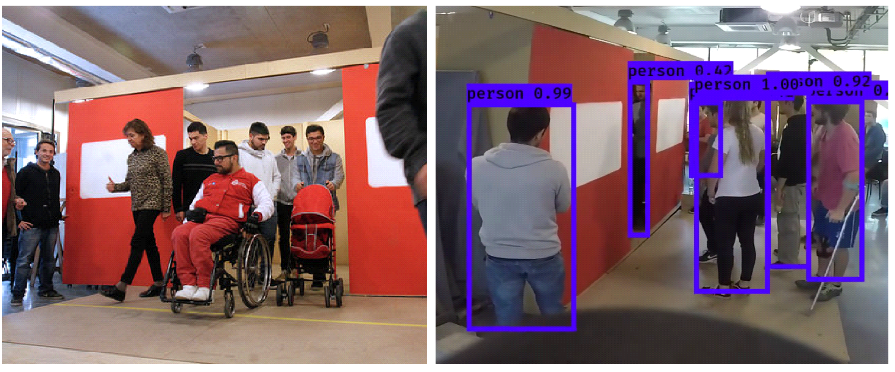
\includegraphics[width=0.8\textwidth]{imagenes/ilustracion_4.png}
  \caption{Tabla Nivel de cumplimiento por parte de los pasajeros (adaptado de Metro de Londres, 2015)
  }\label{fig4}
\end{figure}
